\documentclass{article}
\usepackage{listings}
\usepackage{xcolor}
\usepackage[a4paper, margin=0.5in]{geometry}
\usepackage{graphicx} 

\usepackage{xcolor} 
\definecolor{stronggreen}{rgb}{0.0, 0.5, 0.0}

\pagestyle{empty}

\lstset{
	language=C++,               % Lenguaje de programación
	basicstyle=\ttfamily,       % Tipo de letra
	keywordstyle=\color{blue},  % Palabras clave en azul
	commentstyle=\color{stronggreen}, % Comentarios en verde
	stringstyle=\color{red},    % Cadenas en rojo
	numbers=left,               % Numeración de líneas
	numberstyle=\tiny\color{gray}, % Estilo de numeración
	stepnumber=1,               % Paso de numeración
	numbersep=5pt,              % Separación de la numeración del código
	showspaces=false,           % No mostrar espacios
	showstringspaces=false,     % No mostrar espacios en cadenas
	showtabs=false,             % No mostrar tabulaciones
	frame=single,               % Borde del código
	tabsize=2,                  % Tamaño de la tabulación
	breaklines=true,            % Ajustar líneas largas
	breakatwhitespace=true,     % Romper líneas en espacios
	title=\lstname              % Mostrar el nombre del archivo como título
}
\begin{document}
	
	
\section*{Plantilla de código}

\begin{lstlisting}[language=C++]
	#include <bits/stdc++.h>
	using namespace std; 
	
	#define all(v) v.begin(),v.end()
	#define rall(v) v.rbegin(),v.rend()
	#define pb push_back
	#define mp make_pair
	#define fi first
	#define se second
	typedef long long ll; 
	typedef vector<int> vi; 
	typedef vector<ll> vll; 
	typedef vector<vi> vvi; 
	typedef pair<int,int> ii; 
	void read_vi(vi &a, int n){for(int i=0; i<n; i++) cin >> a[i];}
	void read_vll(vll &a, int n){for(int i=0; i<n; i++) cin >> a[i];}
	
	void solve(){
		
	}
	
	int main(){
		ios_base::sync_with_stdio(false);
		cin.tie(0); cout.tie(0); 
		
		int t = 1; 
		cin >> t; 
		
		while(t--){
			solve(); 
		}
		
		return 0; 
	}
\end{lstlisting}

	
	\newpage
	
	

\begin{figure}[h]
	\centering
	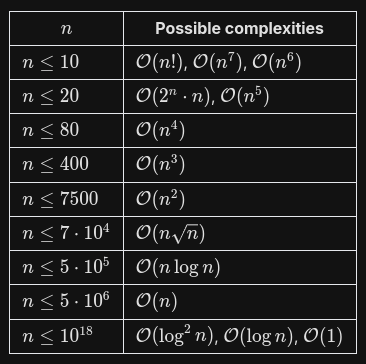
\includegraphics[width=0.6\textwidth]{images/complexities.png}
\end{figure}

\vspace{1cm}

\begin{figure}[h]
	\centering
	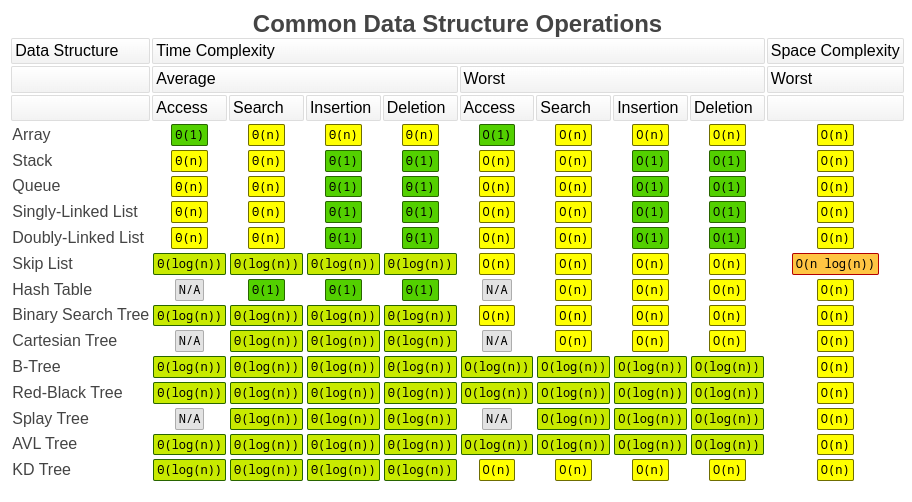
\includegraphics[width=0.8\textwidth]{images/dsComplexities.png}
\end{figure}
	
	\newpage
	
	
\section*{Vector}

\begin{lstlisting}[language=C++]
	#include <bits/stdc++.h>
	using namespace std;
	
	int main() {
		vector<int> vec;
		
		// Anadir elementos
		vec.push_back(10); // [10]
		vec.push_back(20); // [10, 20]
		
		// Acceder a elementos
		cout << vec[0] << endl; // 10
		
		// Eliminar el ultimo elemento
		vec.pop_back(); // [10]
		
		// Tamano del vector
		cout << vec.size() << "\n"; // 1
		
		// Vaciar el vector
		vec.clear();
		
		cout << "Vector vacio: " << (vec.empty() ? "Si" : "No") << endl;
		return 0;
	}
\end{lstlisting}

	\newpage
	
'\section*{List}

\begin{lstlisting}[language=C++]
	#include <bits/stdc++.h>
	using namespace std;
	
	int main() {
		list<int> lst; // []
		
		// Anadir elementos al final
		lst.push_back(10); // [10]
		lst.push_back(20); // [10, 20]
		
		// Anadir elementos al inicio
		lst.push_front(30); // [30, 10, 20]
		
		// Acceder al primer elemento
		cout << lst.front() << "\n"; // 30
		
		// Acceder al ultimo elemento
		cout << lst.back() << "\n"; // 20
		
		// Elimina el primer elemento
		lst.pop_front(); // [10, 20]
		
		// Elimina el ultimo elemento
		lst.pop_back(); // [10]
		
		// Tamano de la lista
		cout << lst.size() << "\n"; // 1
		
		// Vaciar la lista
		lst.clear();
		
		cout << "Lista vacia: " << (lst.empty() ? "Si" : "No") << "\n";
		
		return 0;
	}
\end{lstlisting}

	\newpage
	
\section*{Deque}

\begin{lstlisting}[language=C++]
	#include <bits/stdc++.h>
	using namespace std;
	
	int main() {
		deque<int> deq; //[]
		
		// Anadir elementos al final 
		deq.push_back(10); // [10]
		deq.push_back(20); // [10, 20]
		
		// Anadir elementos al inicio
		deq.push_front(30); // [30, 10, 20]
		
		// Acceder al primer elemento 
		cout << deq.front() << "\n"; // 30
		
		// Acceder al ultimo elemento 
		cout << deq.back() << "\n"; // 20
		
		// Elimina el primer elemento 
		deq.pop_front(); // [10, 20]
		
		// Elimina el ultimo elemento 
		deq.pop_back(); // [10]
		
		// Tamano de la deque
		cout << deq.size() << "\n"; // 1
		
		// Vaciar la deque
		deq.clear();
		
		cout << "Deque vacio: " << (deq.empty() ? "Si" : "No") << "\n";
		
		return 0;
	}
\end{lstlisting}

	\newpage
	
\section*{Map}

\begin{lstlisting}[language=C++]
	#include <bits/stdc++.h>
	using namespace std;
	
	int main() {
		map<int, string> m; // []
		
		// Insertar elementos
		m[1] = "uno"; // [1->uno]
		m[2] = "dos"; // [1->uno, 2->dos]
		m[3] = "tres"; // [1->uno, 2->dos, 3->tres]
		
		// Acceder a un valor usando una clave
		cout << m[2] << "\n"; // dos
		
		// Iterar sobre el mapa e imprimir pares clave-valor
		for (const auto& p : m) {
			cout << p.first << " -> " << p.second << "\n";
		}
		
		// Usar count para verificar la existencia de una clave
		cout << m.count(2) << "\n"; // 1
		cout << m.count(4) << "\n"; // 0
		
		// Eliminar un elemento por clave
		m.erase(2); // [1->uno, 3->tres]
		
		// Verificar existencia de un elemento despues de eliminar
		if (m.find(2) == m.end()) {
			cout << "Elemento encontrado.\n"; 
		}
		
		// Usar iterador para eliminar un elemento
		auto it = m.find(3); 
		if (it != m.end()) {
			m.erase(it);  // [1->uno]
		}
		
		// Tamano del mapa
		cout << m.size() << "\n"; // 1
		
		// Vaciar el mapa
		m.clear();
		
		cout << "Mapa vacio: " << (m.empty() ? "Si" : "No") << "\n"; // Si
		
		return 0;
	}
\end{lstlisting}

	\newpage
	
\section*{Set}

\begin{lstlisting}[language=C++]
	#include <bits/stdc++.h>
	using namespace std;
	
	int main() {
		set<int> s; // []
		
		// Insertar elementos
		
		s.insert(40); // [40]
		s.insert(10); // [10, 40]
		s.insert(20); // [10, 20, 40]
		s.insert(30); // [10, 20, 30, 40]
		s.insert(50); // [10, 20, 30, 40, 50]
		
		// Acceder e imprimir elementos
		for (const auto& elem : s) {
			cout << elem << " ";
		}
		cout << "\n";
		
		// Obtener el primer elemento
		cout << *s.begin() << "\n"; // 10
		
		// Obtener el ultimo elemento
		cout << *prev(s.end()) << "\n"; // 50
		
		// Usar count para verificar la existencia de un elemento
		cout << s.count(20) << "\n"; // 1
		cout << s.count(60) << "\n"; // 0
		
		// Eliminar un elemento
		s.erase(20); // [10, 30, 40, 50]
		
		// Verificar existencia de un elemento despues de eliminar
		if (s.find(20) == s.end()) {
			cout << "Elemento no encontrado.\n"; 
		}
		
		// Tamano del conjunto
		cout << s.size() << "\n"; // 4
		
		// Vaciar el conjunto
		s.clear();
		
		cout << "Conjunto vacio: " << (s.empty() ? "Si" : "No") << "\n"; // Si
		
		return 0;
	}
	
\end{lstlisting}

	\newpage
	
'\section*{Multiset}

\begin{lstlisting}[language=C++]
	#include <bits/stdc++.h>
	using namespace std;
	
	int main() {
		multiset<int> ms; // []
		
		// Insertar elementos
		ms.insert(10); // [10]
		ms.insert(20); // [10, 20]
		ms.insert(10); // [10, 10, 20]
		ms.insert(30); // [10, 10, 20, 30]
		ms.insert(20); // [10, 10, 20, 20, 30]
		ms.insert(40); // [10, 10, 20, 20, 30, 40]
		ms.insert(20); // [10, 10, 20, 20, 20, 30, 40]
		ms.insert(50); // [10, 10, 20, 20, 30, 40, 50]
		
		// Acceder e imprimir elementos
		for (const auto& elem : ms) {
			cout << elem << " ";
		}
		cout << "\n";
		
		// Obtener el primer elemento
		cout << *ms.begin() << "\n"; // 10
		
		// Obtener el ultimo elemento
		cout << *prev(ms.end()) << "\n"; // 50
		
		// Usar count para verificar la existencia y la cantidad de un elemento
		cout << ms.count(20) << "\n"; // 3
		cout << ms.count(60) << "\n"; // 0
		
		// Eliminar un elemento (elimina solo una instancia si hay duplicados)
		auto it = ms.find(20); 
		if(it != ms.end()){
			ms.erase(it); // [10, 10, 20, 20, 30, 40, 50]
		}
		
		// Eliminar todas las instancias de un elemento
		ms.erase(10); // [20, 20, 30, 40, 50]
		
		// Verificar existencia de un elemento despues de eliminar
		if (ms.find(10) == ms.end()) {
			cout << "Elemento no encontrado.\n"; 
		}
		
		cout << ms.size() << "\n"; // 4
		
		// Vaciar el multiconjunto
		ms.clear();
		
		cout << (ms.empty() ? "Si" : "No") << "\n"; // Si
		
		return 0;
	}
	
\end{lstlisting}

	\newpage
	
\section*{Priority Queue}

\begin{lstlisting}[language=C++]
	#include <bits/stdc++.h>
	using namespace std;
	
	int main() {
		priority_queue<int> pq; // es un heap maximo
		
		// Insertar elementos
		pq.push(10); 
		pq.push(30);
		pq.push(20);
		pq.push(5);
		pq.push(25);
		
		// Imprimir el contenido de la priority_queue
		while (!pq.empty()) {
			cout << pq.top() << " "; // Mostrar el elemento con la maxima prioridad
			pq.pop(); // Eliminar el elemento con la maxima prioridad
		}
		cout << "\n";
		
		// Insertar elementos en una priority_queue de prioridad minima (min-heap)
		priority_queue<int, vector<int>, greater<int>> min_pq; // Min-heap
		
		min_pq.push(10);
		min_pq.push(30);
		min_pq.push(20);
		min_pq.push(5);
		min_pq.push(25);
		
		// Imprimir el contenido de la min-heap priority_queue
		while (!min_pq.empty()) {
			cout << min_pq.top() << " "; // Mostrar el elemento con la minima prioridad
			min_pq.pop(); // Eliminar el elemento con la minima prioridad
		}
		cout << "\n";
		
		return 0;
	}

\end{lstlisting}

	\newpage
	
'\section*{Stack}

\begin{lstlisting}[language=C++]
	#include <bits/stdc++.h>
	using namespace std;
	
	int main() {
		stack<int> s; // []
		
		// Insertar elementos en la pila
		s.push(10); // [10]
		s.push(20); // [10, 20]
		s.push(30); // [10, 20, 30]
		s.push(40); // [10, 20, 30, 40]
		
		// Acceder al elemento superior de la pila
		cout << s.top() << "\n"; // 40
		
		// Eliminar el elemento superior de la pila
		s.pop(); // Elimina 40
		
		// Tamano de la pila
		cout << s.size() << "\n"; // 3
		
		// Imprimir el contenido de la pila e irlos eliminando 
		while (!s.empty()) {
			cout << s.top() << " "; 
			s.pop(); 
		}
		cout << "\n"; 
		
		cout << (s.empty() ? "Si" : "No") << "\n"; // Si
		
		return 0;
	}

\end{lstlisting}

	\newpage
	
\section*{Algorithms}

\begin{lstlisting}[language=C++]
	#include <bits/stdc++.h>
	using namespace std;
	
	int main() {
		
		// std::find
		vector<int> vec = {10, 20, 30, 40, 50};
		auto it = find(vec.begin(), vec.end(), 30);
		if (it != vec.end()) {
			cout << "Posicion: " << distance(vec.begin(), it) << "\n"; // 2
		} else {
			cout << "No encontrado.\n";
		}
		
		// std::lower_bound
		sort(vec.begin(), vec.end()); // Necesario para usar lower_bound 
		auto lb = lower_bound(vec.begin(), vec.end(), 35);
		cout << "Primer elemento >= 35: " << (lb != vec.end() ? to_string(*lb) : "No encontrado") << "\n"; // 40
		
		// std::upper_bound
		auto ub = upper_bound(vec.begin(), vec.end(), 35);
		cout << "Primer elemento > 35: " << (ub != vec.end() ? to_string(*ub) : "No encontrado") << "\n"; // 40
		
		// std::binary_search
		bool found = binary_search(vec.begin(), vec.end(), 40);
		cout << (found ? "encontrado" : "no encontrado") << "\n";
		
		// std::sort (ascendente)
		vector<int> unsorted = {5, 3, 8, 6, 2}; // [2, 3, 5, 6, 8]
		sort(unsorted.begin(), unsorted.end());
		
		// std::sort (descendente)
		sort(unsorted.begin(), unsorted.end(), greater<int>()); // [8, 6, 5, 3, 2]
		
		// std::swap
		vector<int> swp = {10, 20, 30, 40, 50};
		swap(swp[0], swp[4]); // [50, 20, 30, 40, 10]
		
		// std::reverse
		vector<int> to_reverse = {1, 2, 3, 4, 5};
		reverse(to_reverse.begin(), to_reverse.end()); // [5, 4, 3, 2, 1]
		
		return 0;
	}
\end{lstlisting}

	\newpage
	
\section*{Strings}

\begin{lstlisting}[language=C++]
	#include <bits/stdc++.h>
	using namespace std;
	
	int main() {
		
		string s1 = "Hello World";
		string s2 = s1; 
		
		char c1 = s1[0]; // Primer caracter
		
		// Manipulacion de cadenas
		
		s1.append(" hi"); // s1 = "Hello World hi"
		s1 = s2; 
		
		s1.append(" Wonderful", 8); // Anade los primeros 8 caracteres de la cadena " Wonderful", s1 = "Hello World Wonderf"
		s1 = s2;
		
		s1.append(5, '!'); // s1 = Hello!!!!!
		s1 = s2; 
		
		s1.insert(6, "Beautiful"); // Insertar en la posicion 6, s1 = "Hello BeautifulWorld"
		s1 = s2; 
		
		s1.erase(6, 10); // Borrar 10 caracteres desde la posicion 6, s1 = "Hello "
		s1 = s2; 
		
		string sub = s1.substr(6, 7); // Extraer subcadena de 7 caracteres desde la posicion 6, sub = "World"
		
		// Busqueda y comparacion
		size_t pos1 = s1.find("Amazing"); // Encontrar "Amazing"
		size_t pos2 = s1.rfind("a"); // Encontrar la ultima aparicion de 'a'
		
		if (pos1 != string::npos) {
			cout << "Encontrado 'Amazing' en la posicion: " << pos1 << "\n";
		} else {
			cout << "'Amazing' no encontrado\n";
		}
		
		if (pos2 != string::npos) {
			cout << "Ultima aparicion de 'a' en la posicion: " << pos2 << "\n";
		} else {
			cout << "'a' no encontrado\n";
		}
		
		// Comparacion de cadenas
		int compareResult = s1.compare("Hello Amazing");
		if (compareResult == 0) {
			cout << "Las cadenas son iguales\n";
		} else if (compareResult < 0) {
			cout << "s1 es menor que 'Hello Amazing'\n";
		} else {
			cout << "s1 es mayor que 'Hello Amazing'\n";
		}
		
		// Transformaciones y limpieza
		transform(s1.begin(), s1.end(), s1.begin(), ::tolower); // Convertir a minusculas
		
		// Convertir de nuevo a mayusculas
		transform(s1.begin(), s1.end(), s1.begin(), ::toupper);
		
		// Espacios y otros caracteres no deseados
		s1.erase(remove_if(s1.begin(), s1.end(), ::isspace), s1.end()); // Eliminar espacios
		
		
		// Conversiones
		string intStr = "12345";
		string longStr = "123456789012345";
		
		// Convertir cadena a entero (int)
		int intVal = stoi(intStr);
		
		// Convertir cadena a entero largo largo (long long)
		long long longLongVal = stoll(longStr);
		
		if (islower('a')) 
			// Es una letra minuscula
		
		if (isupper('A')) 
			// Es una letra mayuscula
		
		if (isdigit('5')) 
			// Es un digito
			
		if (isalpha('A')) 
			// Es una letra
			
		if (isalnum('1')) 
			// Es alfanumerico
			
		if (ispunct('!')) 
			// Es un signo de puntuacion
			
		char c = tolower('A'); // 'a'
		
		char c = toupper('a'); // 'A'
		
		return 0;
	}
\end{lstlisting}

	\newpage
	
\section*{Binary Search}

\begin{lstlisting}[language=C++]
#include <bits/stdc++.h>
using namespace std;

int binarySearch(vector<int>& arr, int low, int high, int x) {
	while (low <= high) {
		int mid = low + (high - low) / 2;
		
		// Verifica si x esta presente en mid
		if (arr[mid] == x)
		return mid;
		
		// Si x es mayor, ignorar la mitad izquierda
		if (arr[mid] < x)
		low = mid + 1;
		// Si x es menor, ignorar la mitad derecha
		else
		high = mid - 1;
	}
	
	// Si llegamos aqui, el elemento no estaba presente
	return -1;
}

int main() {
	vector<int> arr = {2, 3, 4, 10, 40};
	int x = 10;
	int result = binarySearch(arr, 0, arr.size() - 1, x);
	
	// Mostrar el resultado
	if (result == -1) {
		cout << "El elemento no esta presente en el arreglo." << endl;
	} else {
		cout << "El elemento esta presente en el indice " << result << "." << endl; // 0 indezado
	}
	return 0;
}
\end{lstlisting}

	\newpage
	
\section*{KMP Algorithm for Pattern Searching}

\begin{lstlisting}[language=C++]
#include <bits/stdc++.h>
using namespace std;

void computeLPSArray(string& pat, int M, vector<int>& lps)
{
	int len = 0;
	lps[0] = 0;
	
	int i = 1;
	while (i < M) {
		if (pat[i] == pat[len]) {
			len++;
			lps[i] = len;
			i++;
		}
		else 
		{
			if (len != 0) {
				len = lps[len - 1];
			}
			else
			{
				lps[i] = 0;
				i++;
			}
		}
	}
}

vector<int> KMPSearch(string& pat, string& txt)
{
	int M = pat.length();
	int N = txt.length();
	
	vector<int> lps(M);
	vector<int> result;
	
	computeLPSArray(pat, M, lps);
	
	int i = 0; 
	int j = 0; 
	while ((N - i) >= (M - j)) {
		if (pat[j] == txt[i]) {
			j++;
			i++;
		}
		
		if (j == M) {
			result.push_back(i - j + 1);
			j = lps[j - 1];
		}
		else if (i < N && pat[j] != txt[i]) {
			if (j != 0)
			j = lps[j - 1];
			else
			i = i + 1;
		}
	}
	return result;
}

int main()
{
	string txt = "geeksforgeeks";
	string pat = "geeks";
	
	// Vector con los indices donde se encuentra la cadena pat (1-indexado)
	vector<int> result = KMPSearch(pat, txt);
	
	for (int i = 0; i < result.size(); i++) {
		cout << result[i] << " "; // 1 9 
	}
	return 0;
}
\end{lstlisting}
	
	\newpage
	
\section*{Segment Tree}

\begin{lstlisting}[language=C++]
#include <bits/stdc++.h>
using namespace std; 

#define INF INT_MAX
typedef long long ll; 
typedef vector<int> vi; 
typedef vector<ll> vll; 
void read_vi(vi &a, int n){for(int i=0; i<n; i++) cin >> a[i];}


// Implementacion de Segment Tree para encontrar minimos 
class Segment_tree{
	public :
	vll t ;
	
	Segment_tree(int n = 1e5+10){
		t.assign(n*4,INF) ;
	}
	
	void update(int node, int index , int tl , int tr, int val){
		
		if(tr < index || tl > index) return ;
		if(tl == tr){
			t[node] = val ;
		}
		else{
			int mid = tl + ((tr-tl)>>1) ;
			int lft = (node << 1) ;
			int rght = lft + 1;
			
			update(lft,index,tl,mid,val) ;
			update(rght,index,mid+1,tr,val) ;
			t[node] = min(t[lft],t[rght]) ;
		}
		
	}
	
	ll query(int node , int l , int r , int tl , int tr){
		
		if(tl > r || tr < l) return INF ;
		if(tl >= l && tr <= r){
			return t[node];
		}
		else{
			int mid = tl + ((tr-tl)>>1) ;
			int lft = (node << 1) ;
			int rght = lft + 1;
			
			ll q1 = query(lft,l,r,tl,mid) ;
			ll q2 = query(rght,l,r,mid+1,tr) ;
			
			return min(q1,q2) ;
		}
	}
	
	void build(vi &v, int node , int tl , int tr){
		if(tl == tr){
			t[node] = v[tl];
		}
		else{
			int mid = tl + ((tr - tl) >> 1);
			int lft = (node << 1);
			int rght = lft + 1;
			
			build(v,lft,tl,mid);
			build(v,rght,mid+1,tr);
			t[node] = min(t[lft] ,t[rght]);
		}
	}
};


void solve() {
	int n, q; 
	cin >> n >> q; 
	
	vi v = {5, 2, 6, 3, 7};
	
	// Declaracion con n de espacio 
	Segment_tree seg(n);
	
	// Inicializacion, el nodo raiz siempre con indice 1, y los limites del arbol de 0 a n-1
	seg.build(v, 1, 0, n-1); 
	
	while(q--){
		int t;
		cin >> t; 
		
		// Actualizacion
		if(t == 1){
			int k, u; 
			cin >> k >> u; 
			seg.update(1, k-1, 0, n-1, u); 
		}
		
		// Query
		else{
			int a, b; 
			cin >> a >> b; 
			cout << seg.query(1, a-1, b-1, 0, n-1) << "\n"; 
		}
	}
}

int main(){
	ios_base::sync_with_stdio(false);
	cin.tie(0); cout.tie(0); 
	
	int t = 1; 
	
	while(t--){
		solve(); 
	}
	
	return 0; 
}
\end{lstlisting}

	\newpage
	
\section*{Bitset}

\begin{lstlisting}[language=C++]
#include <bits/stdc++.h>
using namespace std; 

int main() {
	bitset<8> bset1;  
	bitset<8> bset2(12); 
	cout << "bset1: " << bset1 << endl;  // Salida: 00000000
	cout << "bset2: " << bset2 << endl;  // Salida: 00001100

	bitset<8> bset3(5);  // 00000101
	cout << "El bit en la posicion 2: " << bset3[2] << endl;  // Salida: 1
	
	bset3.set(2, 0);  // Cambia el bit en la posicion 2 a 0
	cout << "Despues de modificar: " << bset3 << endl;  // Salida: 00000001
	cout << endl;
	
	bitset<8> bset4(string("1100"));  // Inicializa con un valor binario dado como string
	bitset<8> bset5(string("1010"));  
	
	cout << "bset4: " << bset4 << endl;  // Salida: 00001100
	cout << "bset5: " << bset5 << endl;  // Salida: 00001010
	
	cout << "bset4 & bset5: " << (bset4 & bset5) << endl;  // AND: 00001000
	cout << "bset4 | bset5: " << (bset4 | bset5) << endl;  // OR:  00001110
	cout << "bset4 ^ bset5: " << (bset4 ^ bset5) << endl;  // XOR: 00000110
	
	cout << "Todos los bits de bset4 estan en 1? " << (bset4.all() ? "Si" : "No") << endl;  // No
	cout << "Algun bit de bset4 esta en 1? " << (bset4.any() ? "Si" : "No") << endl;  // Si
	cout << "Ningun bit de bset4 esta en 1? " << (bset4.none() ? "Si" : "No") << endl;  // No
	cout << "Numero de bits en 1 en bset4: " << bset4.count() << endl;  // 2
	
	bset4.flip();  // Invierte todos los bits
	cout << "Despues de invertir bset4: " << bset4 << endl;  // Salida: 11110011
	
	bitset<8> bset6(string("10010101"));  // 10010101
	cout << "bset6: " << bset6 << endl;  // Salida: 10010101
	
	// Convertir a unsigned long
	cout << "Como numero entero (unsigned long): " << bset6.to_ulong() << endl;  // Convierte a unsigned long: 149
	
	// Convertir a int (deberas asegurarte de que el valor este dentro del rango de int)
	cout << "Como numero entero (int): " << static_cast<int>(bset6.to_ulong()) << endl;  // Convierte a int: 149
	
	// Convertir a long long
	cout << "Como numero entero (long long): " << static_cast<long long>(bset6.to_ulong()) << endl;  // Convierte a long long: 149
	
	cout << "Como string: " << bset6.to_string() << endl;  // Convierte a string: "10010101"
	
	return 0;
}


\end{lstlisting}

	
\end{document}
